\apendice{Especificación de diseño}

\section{Introducción}
En el presente apartado se detallan los puntos más relevantes en cuanto a los aspectos de diseño de arquitectura, diseño de interfaz y diseño de datos tanto del backend desarrollado en el presente proyecto como de la aplicación que se pretende materializar a futuro.

\section{Diseño de datos}
Para el guardado de la información usamos PostgresSQL. Para ello debimos, primeramente, realizar el trabajo de analizar los requerimientos funcionales y trabajar en cómo se moldearían los datos de los usuarios en el sistema.
Una vez que hicimos este trabajo, utilizando la herramienta \href{https://drive.google.com/file/d/1h34iN2JwS4Tcr9MRbupvjsVVfN3LC1cf/view?usp=sharing}{draw.io}, realizamos el Modelo Entidad Relación donde pudimos establecer cómo se iban a interrelacionar las tablas (ver figura~\ref{Img:Diseno+de+Datos+Backend} y ver figura~\ref{Img:Diseno+de+Datos+Chatbot}).
\begin{figure}[h]
    \centering
    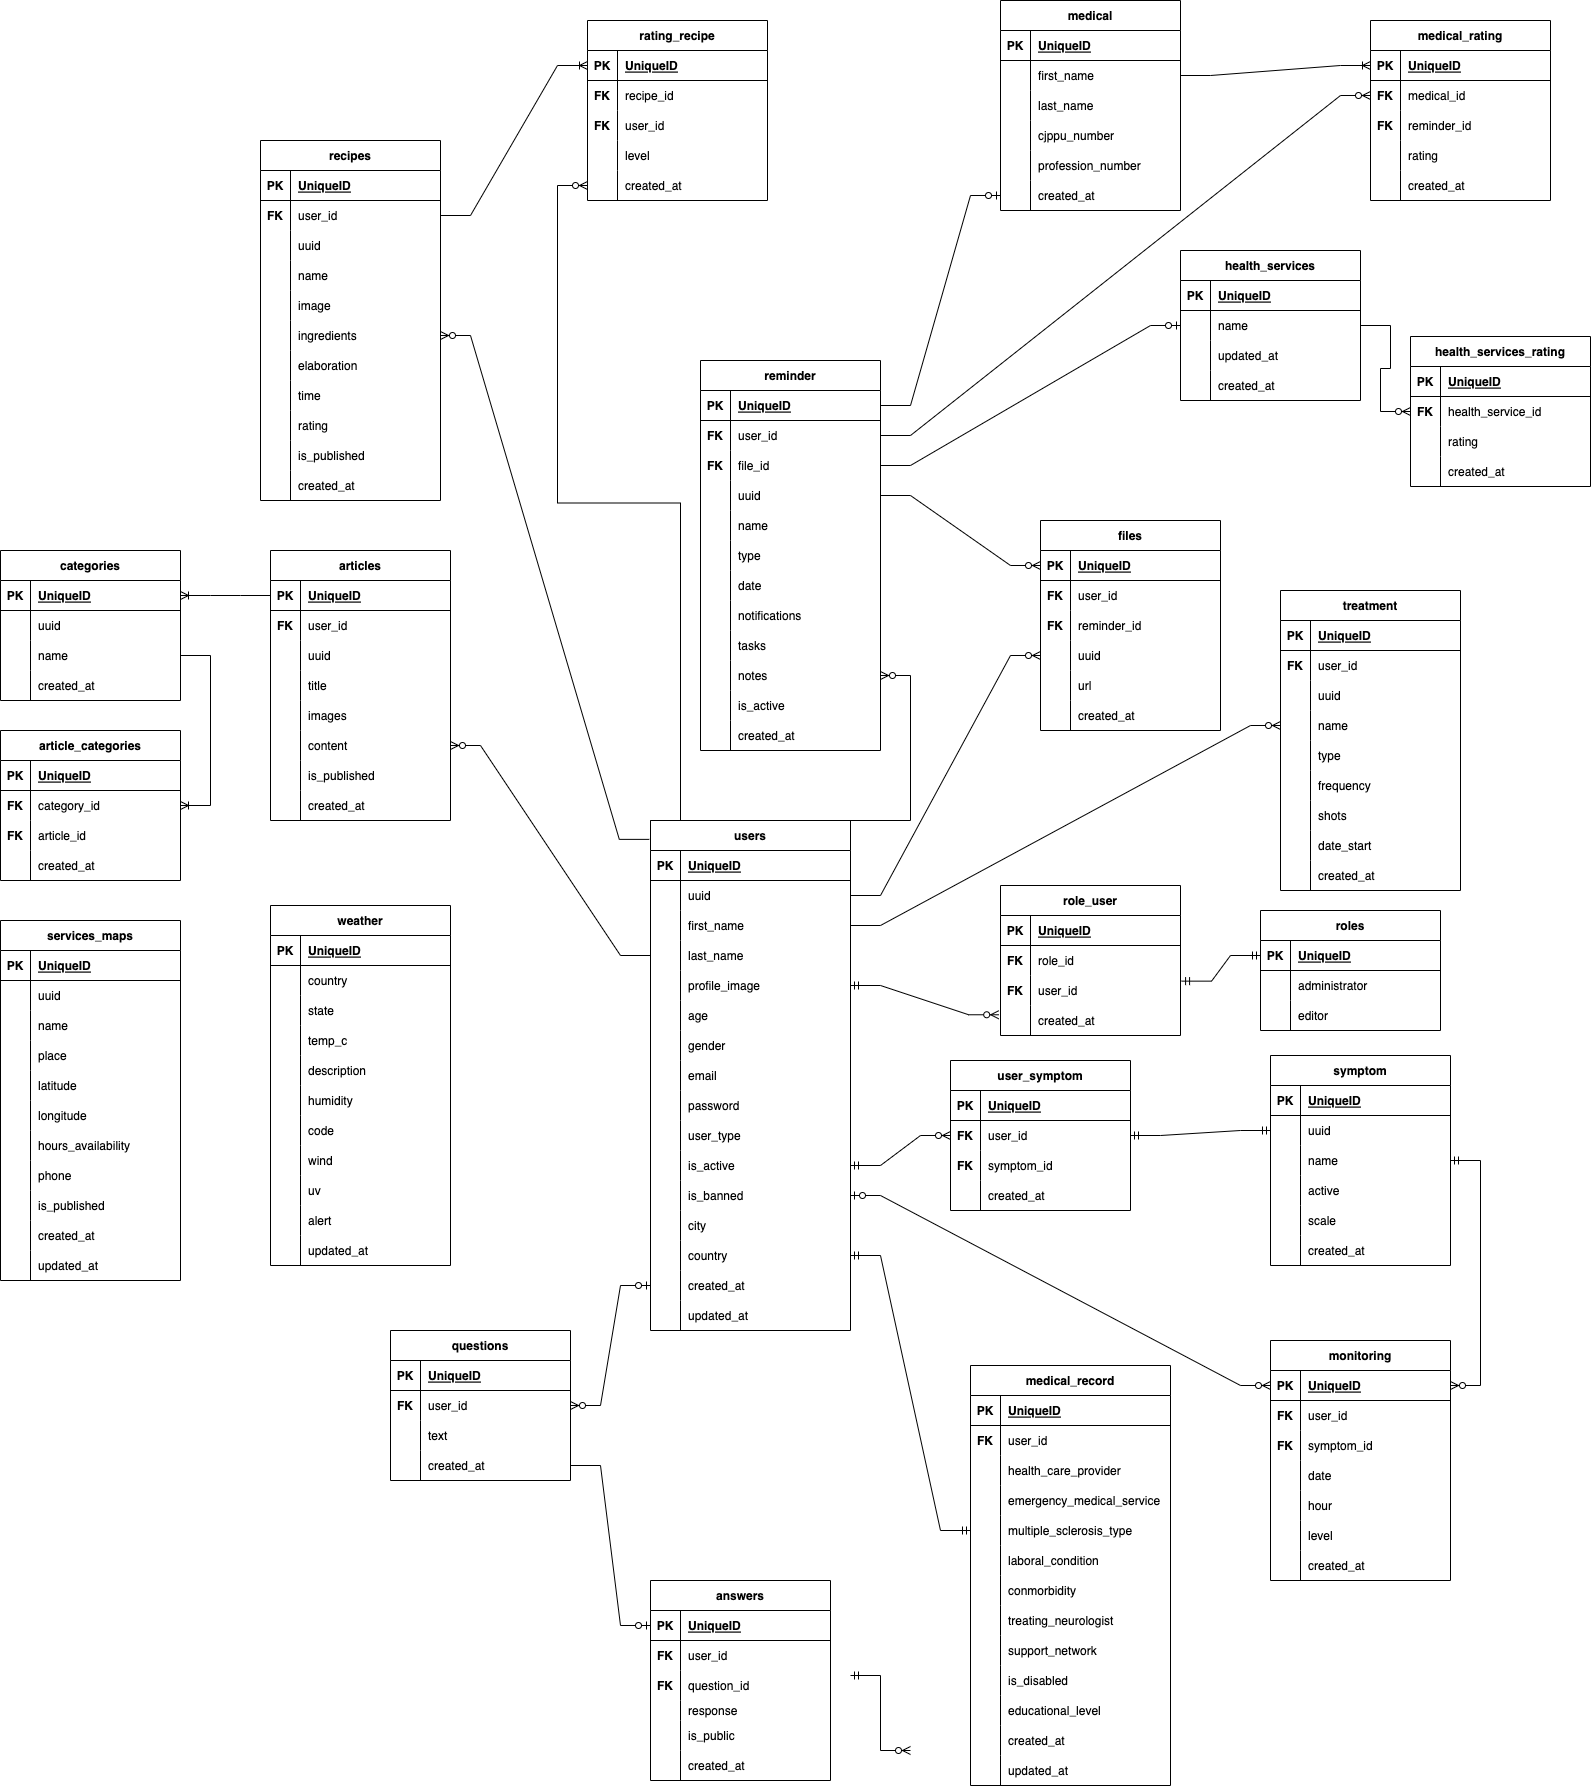
\includegraphics[width=0.7\textwidth]{img/datos/diagrama_db_backend.png}
    \caption{Diagrama MER del backend} \label{Img:Diseno+de+Datos+Backend}
\end{figure} 

\begin{figure}[h]
    \centering
    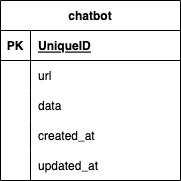
\includegraphics[width=0.3\textwidth]{img/datos/chatbot_emur.drawio.png}
    \caption{Diagrama de tabla para el chatbot} \label{Img:Diseno+de+Datos+Chatbot}
\end{figure} 

\newpage
\section{Diseño procedimental}
A propósito de la arquitectura hexagonal que se ha decidido implementar, se siguió un enfoque modular y basado en la  responsabilidad de cada componente, lo cual incluye controladores (capa de presentación), servicios y puertos que se encuentran en la capa de dominio; por último adaptadores de persistencia ubicados en la capa de datos (ver figura~\ref{Img:Diseno+Procedimental}), el documento original del diagrama también se puede ver en \href{https://drive.google.com/file/d/1Dp13RXxUGILHrhwLvSDbNNQ2T72sM4j7/view?usp=sharing}{draw.io}.

\begin{figure}[h]
    \centering
    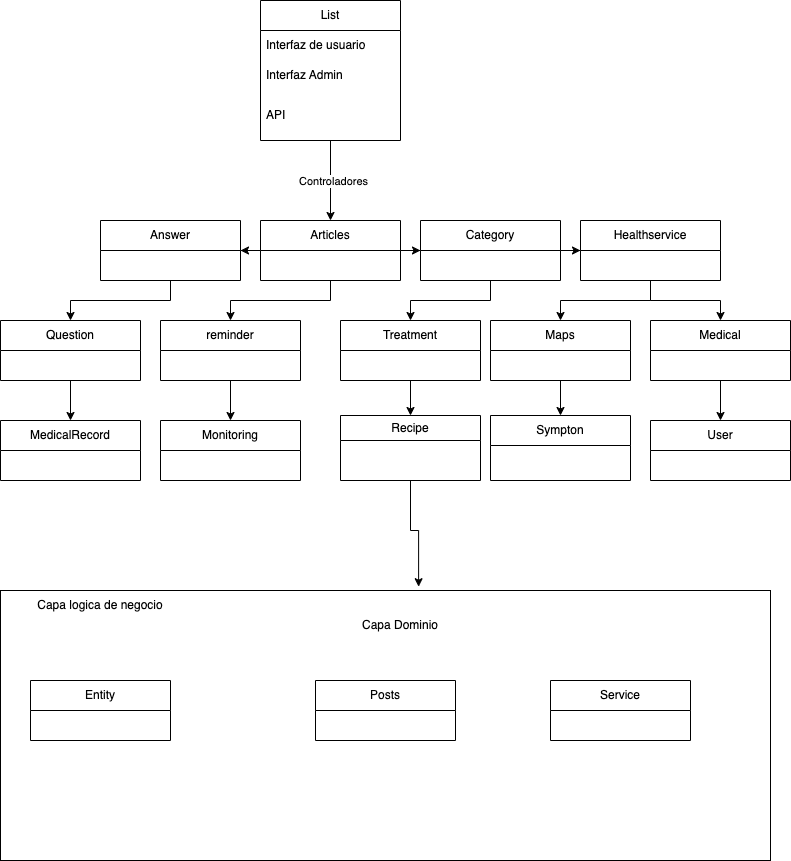
\includegraphics[width=0.7\textwidth]{img/manual/procidemental_drawio.png}
    \caption{Diseño Procedimental} \label{Img:Diseno+Procedimental}
\end{figure} 


\section{Diseño arquitectónico}
A continuación, se presenta la figura~\ref{Img:Diseno+Arquitectura}, donde se aprecia el diseño de arquitectura en el que es posible observar cómo se orquestan los microservicios del backend  y del chatbot para interactuar con la futura aplicación móvil.

\begin{figure}[h]
    \centering
    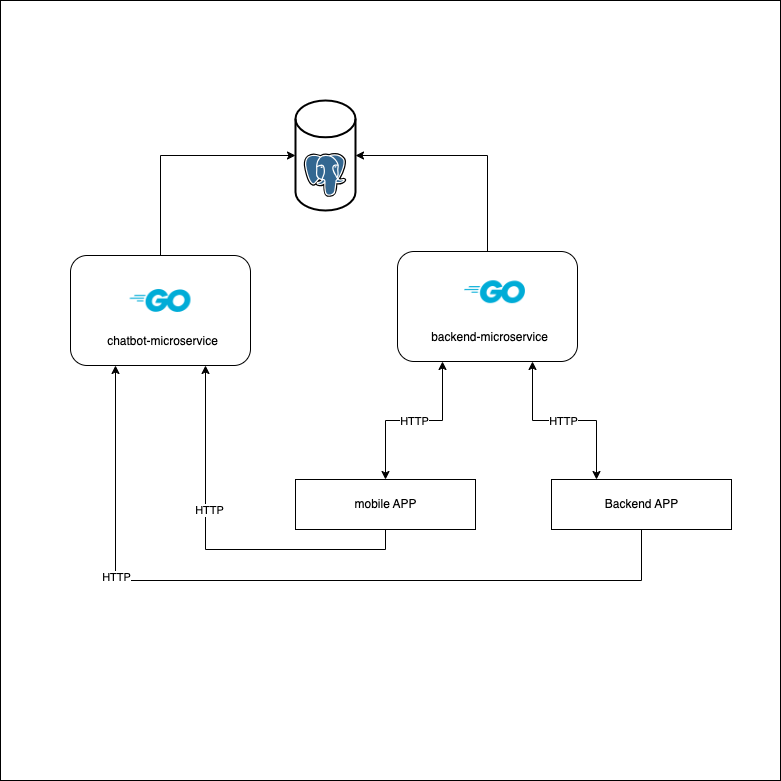
\includegraphics[width=1.0\textwidth]{img/datos/microservices-TFG.drawio.png}
    \caption{Diseño de Arquitectura} \label{Img:Diseno+Arquitectura}
\end{figure} 

\newpage

\section{Diseño de interfaces}

\subsection{Logo para la aplicación móvil a desarrollar a futuro}
Se ha elaborado un logo para la futura aplicación móvil utilizando Adobe Illustrator, conforme puede apreciarse en la figura~\ref{Img:Logo+APP}.

\begin{figure}[h]
    \centering
    
\includegraphics[width=0.4\textwidth]{img/app/red_em.png}
    \caption{Logo propuesto para la aplicación a desarrollar} \label{Img:Logo+APP}
\end{figure} 


\subsection{Interfaz de usuario para la futura aplicación móvil}
Durante la fase de diseño, se elaboraron bocetos digitales sobre cómo debería ser la futura aplicación móvil. Para este fin se utilizó la herramienta Marvel con el fin de poder prototipar las ideas, testearlas y simular su funcionamiento. Se pone a disposición una versión navegable en el siguiente \href{https://marvelapp.com/prototype/c69dgae}{enlace}.

A continuación, es posible observar los prototipos elaborados:

\begin{figure}[h]
    \centering
    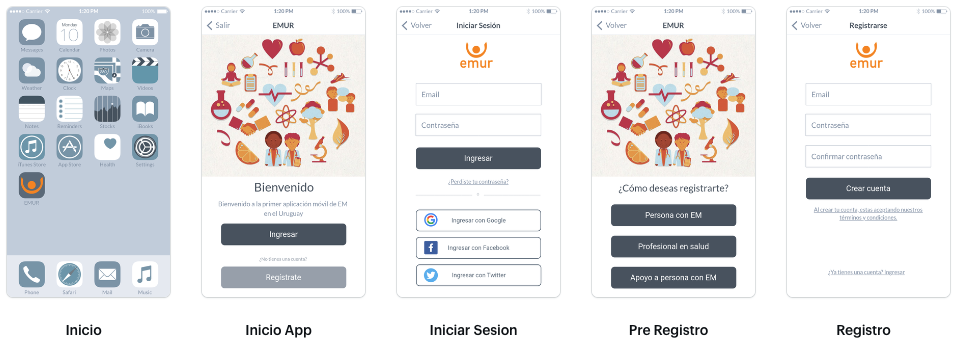
\includegraphics[width=1.1\textwidth]{img/app/diseno_parte1.png}
    \caption{Inicio y Registro} \label{Img:Inicio+Registro}
\end{figure} 

\begin{figure}[h]
    \centering
    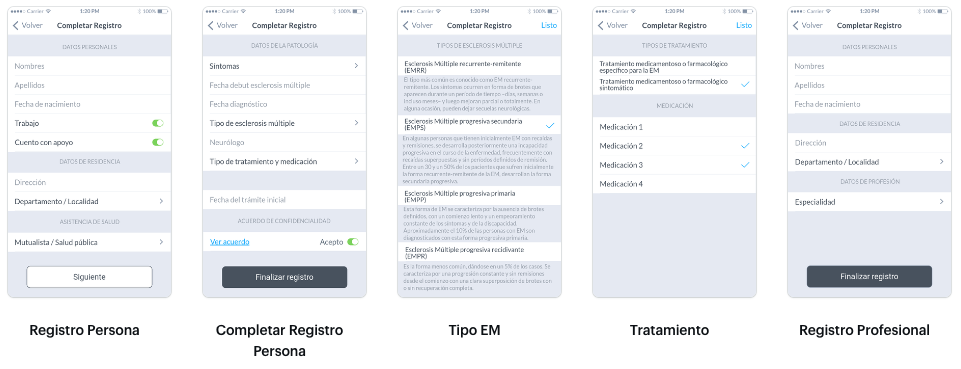
\includegraphics[width=1.1\textwidth]{img/app/diseno_parte2.png}
    \caption{Formularios de Registro} \label{Img:Formularios+Registro}
\end{figure} 

\begin{figure}[h]
    \centering
    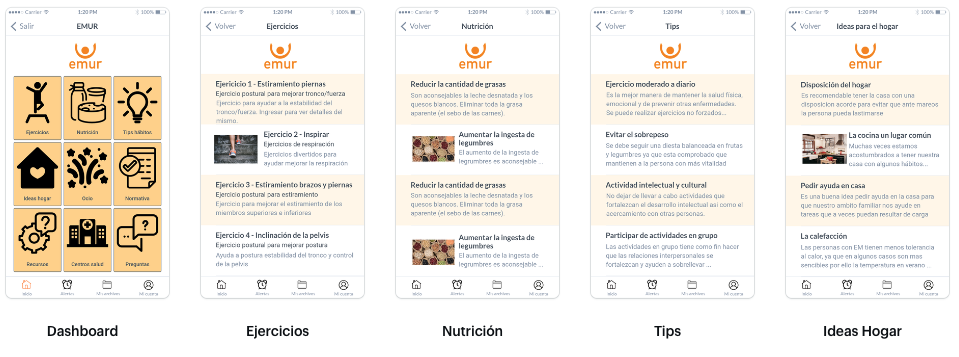
\includegraphics[width=1.1\textwidth]{img/app/diseno_parte3.png}
    \caption{Menú principal y tipos de artículos} \label{Img:Menu+articulos}
\end{figure} 

\begin{figure}[h]
    \centering
    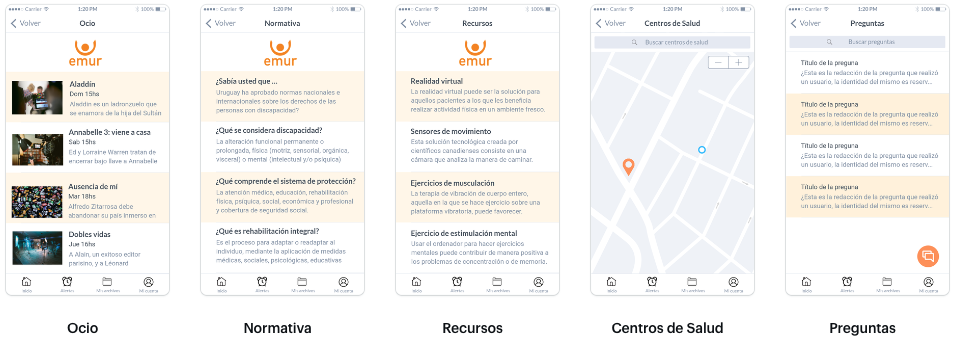
\includegraphics[width=1.1\textwidth]{img/app/diseno_parte4.png}
    \caption{Mapa, Recursos, Vista general de preguntas} \label{Img:Mapa+Recursos}
\end{figure} 

\begin{figure}[h]
    \centering
    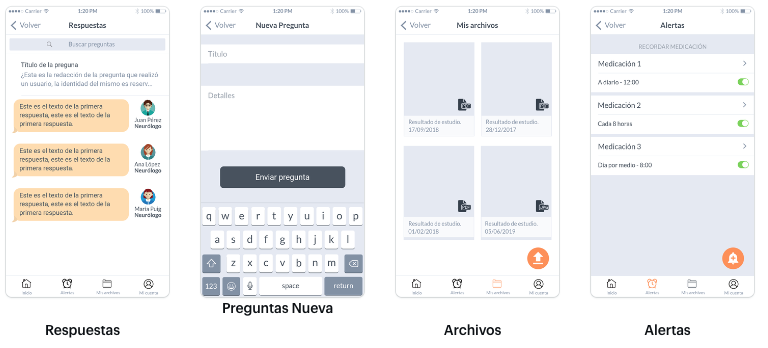
\includegraphics[width=1.1\textwidth]{img/app/diseno_parte5.png}
    \caption{Preguntas y Respuestas, Alertas y Gestión de archivos} \label{Img:Preguntas+Respuestas}
\end{figure} 